%!TEX root = ../../main.tex

Tensors suffer from the infamous \textbf{curse of dimensionality}. This curse
exists because as the number of the dimensions of a tensor grows, its storage
cost and the cost of operations involving it grows exponentially. This is
because the number of entries in a uniform $d$-way tensor is $n^d$. Thus, there
is often a need to compress these large datasets. \textbf{Tensor decompositions}
are techniques that decompose tensors into smaller structured representations.
Similar to most types of matrix decompositions, we seek a set of
matrices/tensors that can be multiplied together appropriately to reconstruct
the input. Matrix or Tensor decompositions can be either exact or
approximations, though the latter is much more common. Most tensor
decompositions can be viewed as higher-order generalizations of matrix
decompositions. There are several types of tensor decompositions, but in this
work we focus on two of the most famous ones; The CP Decomposition, and the
Tucker Decomposition. As mentioned back in the abstract, this thesis is build
upon two projects, each project will focus on one of these decompositions.
Furthermore, though it was just said that exact tensor decompositions are rarer,
the first project focuses on exact CP decompositions of a special type of
tensor. On the other hand, the second project focuses on numeric tensor
approximations using the Tucker Decomposition. 


\subsection{Kruskal Tensors and The CP Decomposition} \label{sec:Kruskal Tensors
    and The CP Decomposition} The CP Decomposition compresses an input tensor
    into a Kruskal Tensor (KTensor), which is a collection of $r$ rank-1
    components. Each component is an outer product of $r$ vectors. We refer to
    $r$ as the rank of the CP decomposition, though this is technically true
    only when $r$ is minimal. The vectors in each mode come together to form a
    factor matrix. We can visualize this in the case of a 3-way tensor as shown
    in \Cref{fig:KTensor}. The rank-1 components in their outer-product format
    are cassually and kindheartdly referred to as chicken feet for their
    appearance. It is crucial to note that we can move these chicken feet around
    as long as we keep their corresponding indeces accross all factor matrices
    together, this fact will be relevant later on.

    \begin{figure}[ht!]
        \centering
        \begin{subfigure}[b]{0.99\textwidth}
            \centering
            % Mess with the first scale to change the size of your drawings
% Mess with the second scale to change the size of your letters
\begin{tikzpicture}[scale=1,namenode/.style={scale=1}]
   % These distances can be meddled with to get you what you want
   % Within reason...
   \def\ix{2.5} %
   \def\iy{2} %
   \def\iz{1.5} %
   \def\rot{90}
   \def\distance{0.75}
   \def\r{0.25} % Thicknesss of chickenfeet
   
   % Give figure's starting point and draw a rectange
   \coordinate (TFrontLowerLeft) at (0,0);
   \draw (TFrontLowerLeft) rectangle ++ (\ix,\iy);

   % This scope draws the top face of the cube
   \begin{scope}[shift={(TFrontLowerLeft)}, canvas is zx plane at y=\iy,rotate=\rot]
      \draw (0,0) rectangle ++ (\ix,\iz);
   \end{scope}

   % This scope draws the left side of the cube
   \begin{scope}[shift={(TFrontLowerLeft)},canvas is zy plane at x=\ix,rotate=90]
      \draw (0,0) rectangle ++ (\iy,\iz); %
   \end{scope}

   % This writes the tensor name in the front face of the cube
   \node[namenode] at ($(TFrontLowerLeft) + (0.5*\ix, 0.5*\iy)$)  {$\mathbf{\mathcal{T}}$};

   % This writes the equal sign to the side of the cube
   \coordinate (ApproxCtr) at ($(TFrontLowerLeft) + (0.75*\distance+\ix+0.5*\iz,0.5*\iy)$);
   \node[namenode] at (ApproxCtr) {=};


   %%%%%%%%% 1st component
   % This draws the vertical chicken feet
   \coordinate (A1LowerLeft) at ($(ApproxCtr) + (\distance,-0.5*\iy)$);
   \draw (A1LowerLeft) rectangle ++ (\r,\iy);
   \node[namenode] at ($(A1LowerLeft) + (\r/2, -0.5*\distance)$) {$\mathbf{a}_1$};

   % This drwas the horizontal chicken feet
   \coordinate (B1LowerLeft) at ($(A1LowerLeft) + (\r + 0.25*\distance,\iy+0.25*\distance)$);
   \draw (B1LowerLeft) rectangle ++ (\ix,\r);
   \node[namenode] at ($(B1LowerLeft) + (0.5*\ix, -0.5*\distance)$) {$\mathbf{b}_1$};

   % This scopee draws the tp-screen chicken feet
   \begin{scope}[shift={($(A1LowerLeft) + (-0.05,2.25*\r)$)},canvas is zx plane at y=\iy,rotate=90]
      \draw (0,\r) rectangle ++ (\r,\iz);
      \node[namenode] at (-0.6*\distance, \iz/1.25) {$\mathbf{c}_1$};
   \end{scope}

   
   % % middle ellipsis
   \coordinate (MiddleEllipsis) at ($(ApproxCtr) + (\r+\ix+3*\distance,0)$);
   % (4*\ix,0.75*\iy);
   \node[namenode] at (MiddleEllipsis) {$+ \quad \cdots \quad +$};
   
   % %%%%%%%%% last component
   \coordinate (ARLowerLeft) at ($(A1LowerLeft) + (\r+\ix+4*\distance,0)$);
   \draw (ARLowerLeft) rectangle ++ (\r,\iy);
   \node[namenode] at ($(ARLowerLeft) + (\r/2, -0.5*\distance)$) {$\mathbf{a}_r$};

   \coordinate (BRLowerLeft) at ($(ARLowerLeft) + (\r + 0.25*\distance,\iy+0.25*\distance)$);
   \draw (BRLowerLeft) rectangle ++ (\ix,\r);
   \node[namenode] at ($(BRLowerLeft) + (0.5*\ix, -0.5*\distance)$) {$\mathbf{b}_r$};

   \begin{scope}[shift={($(ARLowerLeft) + (-0.05,2.25*\r)$)},canvas is zx plane at y=\iy,rotate=90]
      \draw (0,\r) rectangle ++ (\r,\iz);
      \node[namenode] at (-0.6*\distance, \iz/1.25) {$\mathbf{c}_r$};
   \end{scope}

   % \coordinate (OuterProducts) at ($(TFrontLowerLeft) + (\ix+0.4*\iz,0.75*\iy) + (12.75,0)$);
   % \node[namenode] at (OuterProducts) {$\displaystyle = \sum_{i=1}^R \underbrace{\raisebox{0pt}[0pt][10pt]{\mathbf{a}_i \circ \mathbf{b}_i \circ \mathbf{c}_i}}_{\textbf{Outer Products}} = \underbrace{\raisebox{0pt}[0pt][10pt]{\Dsquare{A, B, C}}}_{\textbf{K Tensor}}$};
   
\end{tikzpicture}
            \caption{A 3 way Kruskal Tensor Diagram}
            \label{fig:KTensor}
        \end{subfigure}
        
        \vspace{1em}
        \begin{subfigure}[b]{0.99\textwidth}
            \centering
            \begin{tikzpicture}[scale=1]
   \def\r{4.5}
   \def\ix{2.5}
   \def\iy{2}
   \def\iz{1.5}
   \def\distance{0.25}

   % Vertical bar height (how far above and below the label)
   \def\barheight{0.3}

  % Positions for each matrix
  \def\xA{0}
  \def\xB{\r+0.5}
  \def\xC{2*\r+1}

  % Draw rectangles for A, B, and C
  \draw (\xA,0) rectangle ++(\r,\iy);
  \draw (\xB,0) rectangle ++(\r,\ix);
  \draw (\xC,0) rectangle ++(\r,\iz);

  % Function to draw a vector column with bars above/below
  \newcommand{\vectorcolumn}[4]{
    \draw ({#1}, {#3 + \distance}) -- ({#1}, {#4 - \distance});
    \draw ({#1}, {#3 - \distance}) -- ({#1}, {0 + \distance});
    \node at (#1, #3) {#2};
  }

  % % First two columns: a_1, a_2
  % \foreach \i/\label in {0/1, 1/2} {
  %   \pgfmathsetmacro{\xai}{\xA + (\r/5)*(\i + 0.5)}
  %   \pgfmathsetmacro{\xbi}{\xB + (\r/5)*(\i + 0.5)}
  %   \pgfmathsetmacro{\xci}{\xC + (\r/5)*(\i + 0.5)}
  %   \vectorcolumn{\xai}{$\mathbf{a}_{\label}$}{0.5*\iy}
  %   \vectorcolumn{\xbi}{$\mathbf{b}_{\label}$}{0.5*\ix}
  %   \vectorcolumn{\xci}{$\mathbf{c}_{\label}$}{0.5*\iz}
  % }

  %  % Vector column macro with vertical lines
  %  \newcommand{\vectorcolumn}[5]{ % x, label, y_center, y_top, y_bottom
  %    % Top vertical line
  %    \draw ({#1}, {#3 + #5}) -- ({#1}, {#4 - #5});
  %    % Bottom vertical line
  %    \draw ({#1}, {#3 - #5}) -- ({#1}, {#2 + #5});
  %    % Label node
  %    \node at (#1, #3) {#2};
  %  }

   % First two columns
   \foreach \i/\label in {0/1, 1/2} {
     \pgfmathsetmacro{\xai}{\xA + (\r/5)*(\i + 0.5)}
     \pgfmathsetmacro{\yai}{0.5*\iy}
     \vectorcolumn{\xai}{$\mathbf{a}_{\label}$}{\yai}{\iy} % {\iy}{0.01}{\distance}

     \pgfmathsetmacro{\xbi}{\xB + (\r/5)*(\i + 0.5)}
     \pgfmathsetmacro{\ybi}{0.5*\ix}
     \vectorcolumn{\xbi}{$\mathbf{b}_{\label}$}{\ybi}{\ix} % {\ix}{0}{\distance}

     \pgfmathsetmacro{\xci}{\xC + (\r/5)*(\i + 0.5)}
     \pgfmathsetmacro{\yci}{0.5*\iz}
     \vectorcolumn{\xci}{$\mathbf{c}_{\label}$}{\yci}{\iz} % {\iz}{0}{\distance}
   }

   % Ellipsis column (centered)
   \node at ({\xA + (\r/5)*2.5}, {0.5*\iy}) {\ldots};
   \node at ({\xB + (\r/5)*2.5}, {0.5*\ix}) {\ldots};
   \node at ({\xC + (\r/5)*2.5}, {0.5*\iz}) {\ldots};

   % First two columns
   \foreach \i/\label in {3/{r-1}, 4/r} {
     \pgfmathsetmacro{\xai}{\xA + (\r/5)*(\i + 0.5)}
     \pgfmathsetmacro{\yai}{0.5*\iy}
     \vectorcolumn{\xai}{$\mathbf{a}_{\label}$}{\yai}{\iy} % {\iy}{0.01}{\distance}

     \pgfmathsetmacro{\xbi}{\xB + (\r/5)*(\i + 0.5)}
     \pgfmathsetmacro{\ybi}{0.5*\ix}
     \vectorcolumn{\xbi}{$\mathbf{b}_{\label}$}{\ybi}{\ix} % {\ix}{0}{\distance}

     \pgfmathsetmacro{\xci}{\xC + (\r/5)*(\i + 0.5)}
     \pgfmathsetmacro{\yci}{0.5*\iz}
     \vectorcolumn{\xci}{$\mathbf{c}_{\label}$}{\yci}{\iz} % {\iz}{0}{\distance}
   }

  % Matrix labels
  \node at ({\xA + 0.5*\r}, -0.5) {$\mathbf{A}$};
  \node at ({\xB + 0.5*\r}, -0.5) {$\mathbf{B}$};
  \node at ({\xC + 0.5*\r}, -0.5) {$\mathbf{C}$};

\end{tikzpicture}
            \caption[Kruskal Tensor Factor Matrices]{The vectors of the components of the Kruskal tensor come together to form factor matrices}
            \label{fig:KTensor_factor_matrices}
        \end{subfigure}
        \caption[The CP Decomposition]{The CP Decomposition}
    \end{figure}

    Mathetmatically, given a tensor $\mathcal{T} \in \mathbb{R}^{m\times n\times
    p}$ and decomposition rank $r\in \mathbb{N}$, The goal of a CP Decomposition
    is to find factor matrices $\mathbf{A}\in \mathbb{R}^{m\times r},
    \mathbf{B}\in \mathbb{R}^{n\times r}, \mathbf{C}\in \mathbb{R}^{p\times r}$
    such that 

    \begin{equation}
        t_{ijk} = \sum_{\ell = 1}^{r} a_{i\ell}b_{j\ell}c_{k\ell} \text{, } \forall (i, j, k) \in [m]\times [n]\times [p]
    \end{equation}

    Or alternatively:

    \begin{equation}
        \mathcal{T} \approx \llbracket \mathbf{A, B, C} \rrbracket = \sum_{\ell = 1}^{r} a_\ell \circ b_\ell \circ c_\ell
    \end{equation}

    The memory footprint of a KTensor is $3rn$. The approximation gets more
    accurate as $r$ increases. This is the 2D matrix equivalent of having an
    $n\times n$ matrix approximation to be the outer product of $n \times 1$ two
    vectors. Traditional methods of computing the CP decomposition of a tensor
    are gradient descent and the newton method. The method used in this work is
    a variation of the later called damped gauss newton. All these methods often
    minimize the sum of squares error. The least squares error is shown in
    \ref{eq:cp_least_squares}:

    \begin{equation} \label{eq:cp_least_squares}
        \|\mathcal{T} - \llbracket \mathbf{A, B, C} \rrbracket \|^2 \equiv \sum_{i=1}^{m} \sum_{j=1}^{n} \sum_{k=1}^{p}\left(t_{ijk} - \sum_{\ell=1}^{r} a_{i\ell}b_{j\ell}c_{k\ell} \right)^2
    \end{equation}

    Thus, the CP optimization problem for a given $r$ is shown in
    \ref{eq:cp_opt}. This is a non-convex problem. 

    \begin{equation} \label{eq:cp_opt}
        \min_{A} \|\mathcal{T} - \llbracket \mathbf{A, B, C} \rrbracket \|^2 \text{, subject to } \mathbf{A} \in \mathbb{R}^{m\times r} \mathbf{B} \in \mathbb{R}^{n\times r} \mathbf{C} \in \mathbb{R}^{p\times r}
    \end{equation}
        




\subsection{Tucker Tensors and The Tucker Decomposition} \label{sec:Tucker Tensors and The Tucker Decomposition}
    The Tucker Decomposition compresses an input tensor into a Tucker Tensor
    (TTensor), which is a smaller core tensor with a factor matrix for each of
    its modes. To reconstruct the approximation of the original tensor, each
    factor matrix is multiplied with the core in its respective mode through a
    TTM. We can visualize this in the case of a 3-way tensor as shown in
    \Cref{fig:TTensor}.

    \begin{figure}[ht]
        \centering
        % 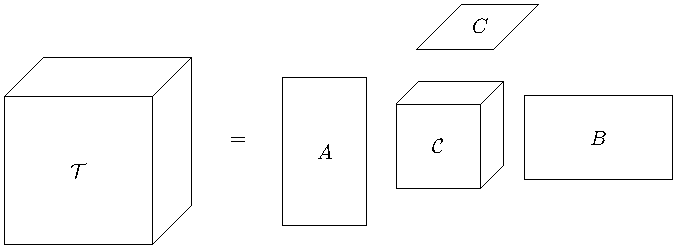
\includegraphics[scale=1]{tikz/chapter1/section1-2/Tucker_Tensor.pdf}
        % Mess with the first scale to change the size of your drawings
% Mess with the second scale to change the size of your letters
\begin{tikzpicture}[scale=1,namenode/.style={scale=1}]
   % These distances can be meddled with to get you what you want
   % Within reason...
   \def\ix{2.5} %
   \def\iy{2.5} %
   \def\iz{1.75} %
   \def\corescale{1.75} % Has to be more than 1
   \def\rot{90}
   \def\r{0.25}
   \def\rx{\ix/\corescale}
   \def\ry{\iy/\corescale}
   \def\rz{\iz/\corescale}
   
   % Give figure's starting point and draw a rectange
   \coordinate (TFrontLowerLeft) at (0,0);
   \draw (TFrontLowerLeft) rectangle ++ (\ix,\iy);

   % This scope draws the top face of the cube
   \begin{scope}[shift={(TFrontLowerLeft)}, canvas is zx plane at y=\iy,rotate=\rot]
      \draw (0,0) rectangle ++ (\ix,\iz);
   \end{scope}

   % This scope draws the left side of the cube
   \begin{scope}[shift={(TFrontLowerLeft)},canvas is zy plane at x=\ix,rotate=90]
      \draw (0,0) rectangle ++ (\iy,\iz); %
   \end{scope}

   % This writes the tensor name in the front face of the cube
   \node[namenode] at ($(TFrontLowerLeft) + (0.5*\ix, 0.5*\iy)$)  {$\mathbf{\mathcal{T}}$};

   % This writes the equal sign to the side of the cube
   \coordinate (ApproxCtr) at ($(TFrontLowerLeft) + (0.75+\ix+0.4*\iz,0.7*\iy)$);
   \node[namenode] at (ApproxCtr) {=};

   % First Factor Matrix
   \coordinate (AFrontLowerLeft) at ($(ApproxCtr) + (0.75,-\ry)$);
   \draw (AFrontLowerLeft) rectangle ++ (\rx,\iy);
   \node[namenode] at ($(AFrontLowerLeft) + (0.5*\rx, 0.5*\iy)$)  {$A$};

   % This scope draws the top face of the cube
   \coordinate (CFrontLowerLeft) at ($(AFrontLowerLeft) + (0.5 + \rx, 0.25*\ix)$);
   \draw (CFrontLowerLeft) rectangle ++ (\rx,\ry);
   
   \begin{scope}[shift={(CFrontLowerLeft)}, canvas is zx plane at y=\ry,rotate=\rot]
      \draw (0,0) rectangle ++ (\rx,\rz);
   \end{scope}

   % This scope draws the left side of the cube
   \begin{scope}[shift={(CFrontLowerLeft)},canvas is zy plane at x=\rx,rotate=90]
      \draw (0,0) rectangle ++ (\ry,\rz); %
   \end{scope}

   % This writes the core name in the front face of the cube
   \node[namenode] at ($(CFrontLowerLeft) + (0.5*\rx, 0.5*\ry)$)  {$\mathbf{\mathcal{G}}$};

   % Second Factor Matrix
   \coordinate (BFrontLowerLeft) at ($(CFrontLowerLeft) + (\rx + 0.75*\rz, 0.15*\rz)$);
   \draw (BFrontLowerLeft) rectangle ++ (\ix,\ry);
   \node[namenode] at ($(BFrontLowerLeft) + (0.5*\ix, 0.5*\ry)$)  {$B$};

   % Third Factor Matrix
   \begin{scope}[shift={($(CFrontLowerLeft) + (0.25*\rz,-0.25*\rz)$)},canvas is zx plane at y=\iy,rotate=90]
      \draw (0,\r) rectangle ++ (\rz*1.3,\iz*1.15);
   \end{scope}
   \node[namenode] at ($(CFrontLowerLeft) + (1*\rx,2.75*\rz)$) {$C$};

   
\end{tikzpicture}
        \caption[A 3-way Tucker Tensor Diagram]{A 3-way Tucker Tensor Diagram}
        \label{fig:TTensor}
    \end{figure}

    If we consider a 3D tensor of size $n^3$ with core of size $r^3$ where $r <
    n$. Then the number of entries of a TTensor is $3rn + r^3$ which is less
    than the original memory footprint and much less if $r \ll n$. The
    reconstruction of the original tensor is performed using TTMs as seen in
    \ref{eq:tucker_ttm}, but if we wish to reconstruct but a single entry then
    we perform \ref{eq:tucker_element}

    \begin{equation} \label{eq:tucker_ttm}
        \mathcal{T} \approx \llbracket \mathcal{G}; \mathbf{A,B,C} \rrbracket = \mathcal{G} \times_1 \mathbf{A} \times_2 \mathbf{B} \times_3 \mathbf{C}
    \end{equation}
    
    \begin{equation} \label{eq:tucker_element}
        t_{ijk} = \sum_{\alpha = 1}^{q} \sum_{\beta = 1}^{r} \sum_{\gamma = 1}^{s} g_{\alpha \beta \gamma}\cdot a_{i\alpha}b_{j\beta}c_{i\gamma}\text{, }\forall (i, j, k) \in [m]\otimes[n]\otimes[p]
    \end{equation}
    
    
    The traditional methods are HOSVD (Higher Order Singular Value
    Decomposition) and STHOSVD (Sequentially Truncated Singular Value
    Decomposition). Though HOOI (Higher Order Orthogonal Iteration) is not as
    traditional, it will be the protagonist for this work. We describe these
    algorithms in \Cref{sec:Tucker Algorithms}
